\documentclass{beamer}
\mode<presentation> {
\usetheme{Madrid}
}

\usepackage{amsmath,amsthm,amssymb,amsfonts,listings,graphicx,caption,subcaption,hyperref} % Allows including images
\usepackage{booktabs} % Allows the use of \toprule, \midrule and \bottomrule in tables

%----------------------------------------------------------------------------------------
%	TITLE PAGE
%----------------------------------------------------------------------------------------

\title[Missing Data]{Monday Group Presentation on Missing Data} % The short title appears at the bottom of every slide, the full title is only on the title page

\author{Sam Shi} % Your name
\institute[Ryerson] % Your institution as it will appear on the bottom of every slide, may be shorthand to save space
{
Ryerson University \\ % Your institution for the title page
\medskip
%\textit{john@smith.com} % Your email address
}
\date{\today} % Date, can be changed to a custom date

\begin{document}

\begin{frame}
\titlepage % Print the title page as the first slide
\end{frame}

\begin{frame}
\frametitle{Overview} % Table of contents slide, comment this block out to remove it
\tableofcontents % Throughout your presentation, if you choose to use \section{} and \subsection{} commands, these will automatically be printed on this slide as an overview of your presentation
\end{frame}

%----------------------------------------------------------------------------------------
%	PRESENTATION SLIDES
%----------------------------------------------------------------------------------------

%------------------------------------------------
\section{Missing data} % Sections can be created in order to organize your presentation into discrete blocks, all sections and subsections are automatically printed in the table of contents as an overview of the talk
%------------------------------------------------

\subsection{Types of Missing Data} % A subsection can be created just before a set of slides with a common theme to further break down your presentation into chunks

\begin{frame}
\frametitle{Types of Missing Data}

supposed you want to model weight $Y$ as a function of gender $X$ and you do a survey asking for $Y$ and $X$, in the end there are some missing values(data point missing or data attribute missing), below are possible scenarios,
\begin{itemize}
\item{Missing completely at random(MCAR)}\\
No particular reasons why the data is missing, such as, it can be someone dropped the survey paper, hard recognizable hand-writting, etc. (data are rarely MCAR) 
\item{Missing at random(MAR)}\\
It can happen that one gender $X$ would less likely to disclose their weight information than the other.
\item{Missing not at random(MNAR)}\\
Missing value itself is related to why it is missing, e.g. a person with higher weight $Y$ would more likely not fill out the weight blank on survey. 
\end{itemize}
\end{frame}

%------------------------------------------------
\subsection{Why it is important}
\fontsize{6pt}{7.2}\selectfont
\begin{frame}
\frametitle{why it is important}
\begin{itemize}
\item {Easy to occur very common}
\begin{figure}[h!]
	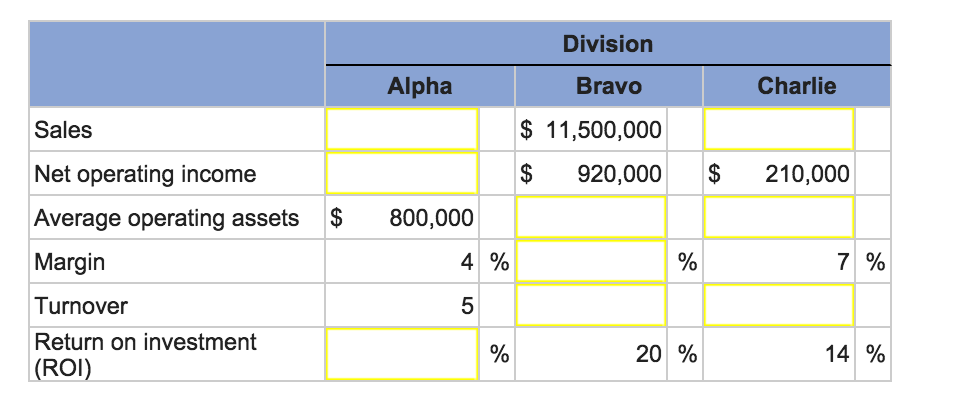
\includegraphics[width=0.2\textwidth]{missing.png}
\end{figure}
\item  Nearly all standard statistical methods presume complete information for
all the variables included in the analysis; Machine learning models need to have complete input.\cite{p1}
\begin{figure}[h!]
	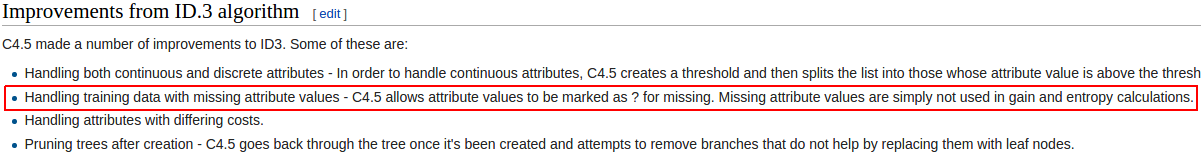
\includegraphics[width=0.6\textwidth]{c45.png}
\end{figure}
\item Create bias \cite{p2}
\begin{figure}[h!]
	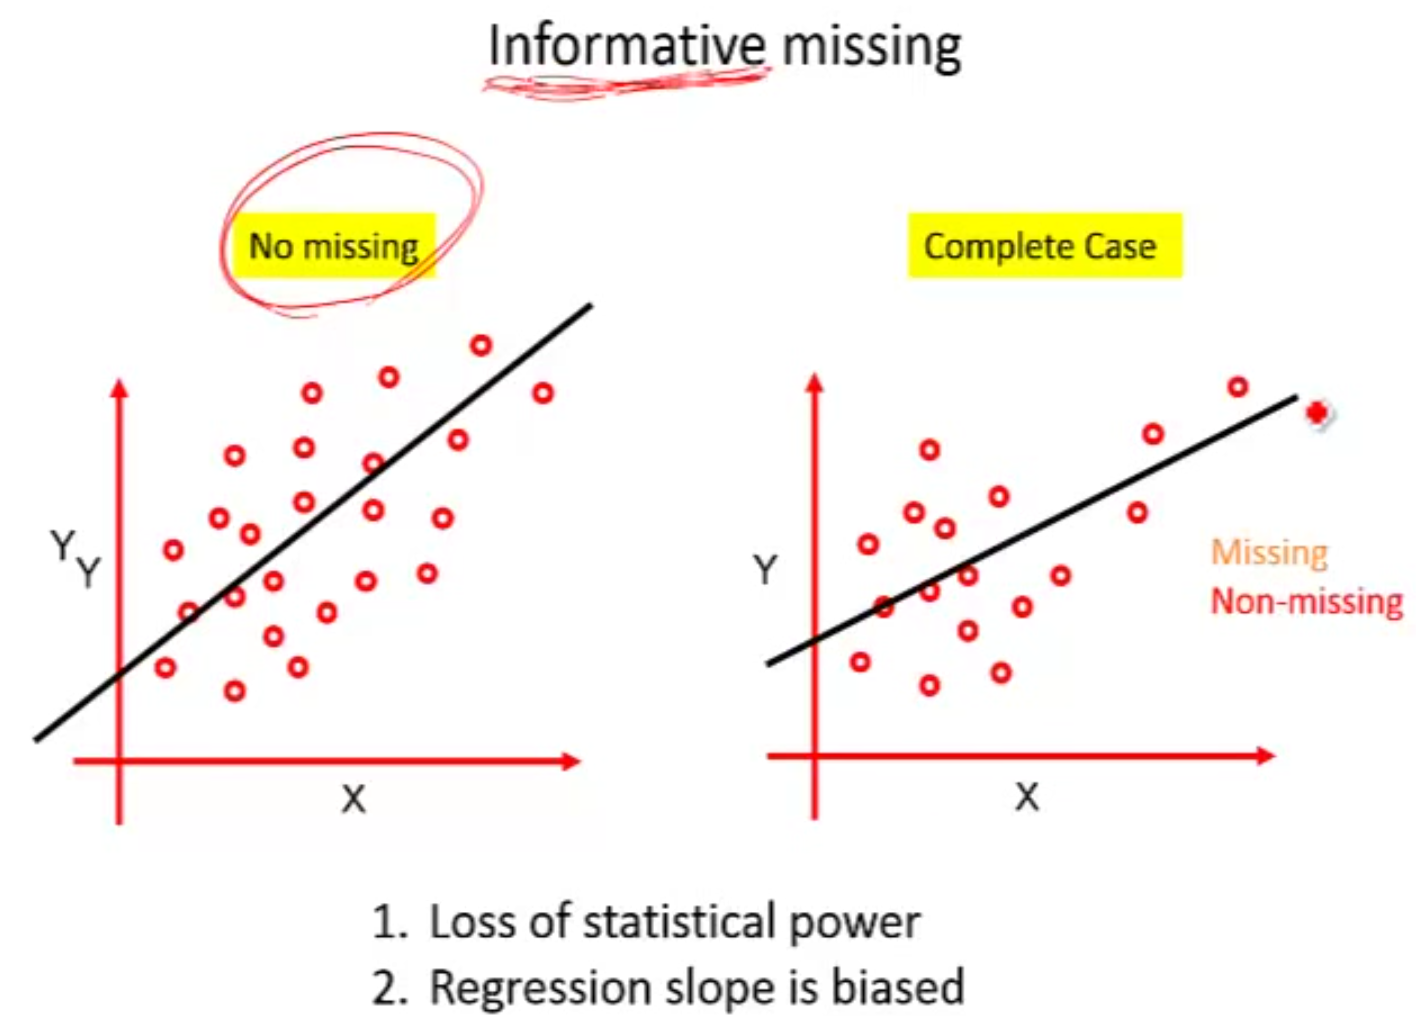
\includegraphics[width=0.5\textwidth]{bias.png}
\end{figure}
\end{itemize}
\end{frame}

%------------------------------------------------
\subsection{Common ways to deal with missing data}
\fontsize{11pt}{7.2}\selectfont
\begin{frame}
\frametitle{Common ways to deal with missing data}
A quick summary before we introudce dealing methods, \cite{p3}\\
	\begin{itemize}
		\item Listwise deletion (or complete case analysis)
		\item Imputation methods
		\item Multiple Imputation
		\item Maximum Likelihood 
		\item Bayesian simulation methods
		\item Hot deck imputation methods
	\end{itemize}
\end{frame}
%------------------------------------------------

\section{Methods}
%------------------------------------------------
\begin{frame}{Listwise deletion}
\begin{columns}[c] 
	
\column{.5\textwidth} % Left column and width
\begin{figure}[h!]
	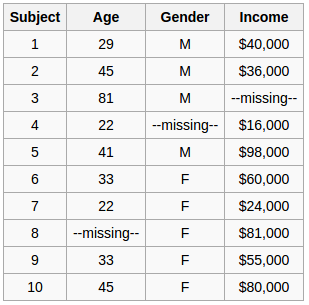
\includegraphics[width=\textwidth]{listwise.png}
\end{figure}
-- picture from Wiki
\column{.5\textwidth} % Right column and width
\textbf{Advantage}:\\
\begin{itemize}
\item{Easy to implement, no special computation metod requires}
\item{It is valid if the missing data is MCAR}
\item{If the proportion of deleted data is small, e.g. $<5\%$}
\end{itemize}
\textbf{Disadvantage}:\\
\begin{itemize}
	\item{Can exclude a large portion of data}
	\item{Missing data are MCAR rarely happens in reality}
	\item{Introduce bias}
\end{itemize}
\end{columns}


\end{frame}
%------------------------------------------------



%------------------------------------------------



%------------------------------------------------

\begin{frame}
\frametitle{References}
\footnotesize{
\begin{thebibliography}{9} % Beamer does not support BibTeX so references must 
\bibitem[Wiki, C4.5]{p1}C4.5: \url{https://en.wikipedia.org/wiki/C4.5_algorithm}
\bibitem[Missing Data Analysis]{p2}Missing Data Analysis: \url{https://www.youtube.com/watch?v=QAvSj2TWZy0}
\bibitem[Computerphile]{p3}The Trouble with Missing Data \url{https://www.youtube.com/watch?v=oCQbC818KKU}
\end{thebibliography}
}
\end{frame}



%----------------------------------------------------------------------------------------

\end{document}